\section{Introduction}

High-dimensional data poses a challenge to traditional likelihood-based modeling approaches.  Penalized regression is an increasingly popular method that is well suited to handle high-dimensional data.  An appealing aspect of many penalized approaches is that they yield sparse models where only a subset of the available variables are ``selected'' by the model in the sense of having non-zero coefficient estimates.  The number of variables in the selected subset can be controlled by changing the degree of penalization, making penalized regression an attractive tool for variable selection in the high-dimensional setting.

Perhaps most popular of these penalized approaches is the least absolute shrinkage and selection operator (lasso) introduced by \citet{tibshirani_1996}. The lasso imposes a penalty on the L1 norm of the estimated regression coefficients that is governed by a single parameter, $\lambda$, such that larger values of $\lambda$ result in more sparse models. In this paper we focus on the variables that are selected by a penalized regression model, in particular we examine how certain are we that these selections are not false discoveries. We do this under the general setting of likelihood-based penalized regression models, which includes GLM and Cox Proportional Hazards models under many popular penalties, including the lasso, SCAD \citep{SCAD}, MCP \citep{MCP}, and elastic net \citep{Elastic_Net}.

To address this question of selection reliability, Breheny (2016) originally proposed a method to estimate marginal false discovery rates for linear lasso regression. Here we begin by outlining this approach, then we extend it to a more general class of regression models.  After doing so, we will compare our estimator's performance with other approaches that are commonly used in high dimensional variable selection.  We conclude by applying our approach to two case studies involving high-dimensional survival and high-dimensional classification data to demonstrate the estimator's practical utility.

\section{Marginal False Discovery Rates}

Consider the causal diagram depicted in Figure~\ref{Fig:diagram}.  In this diagram variable $A$ has a direct causal relationship with the outcome variable $Y$.  Variable $B$ is correlated with variable $Y$, but is not causally related.  Its correlation arises only through its relationship with variable $A$, and if we adjust for variable $A$ there will no longer be any correlation between variable $B$ and the response.  Variable $C$ is clearly uncorrelated with variable $Y$ regardless of which variables our model might adjust for.

\begin{figure}[!htb]
\centering
\begin{tikzpicture}[node distance=1cm]

% nodes %
\node(b)[text centered] {$B$};
\node(u)[below of = b, text centered] {$ $};
\node(a)[left of = u,  text centered, xshift = -1.5cm] {$A$};
\node(c)[right of = u, text centered, xshift = 1.5cm] {$C$};
\node(y)[below of = u, text centered] {$Y$};
 
% edges %
\draw [arrow] (a) -- (b);
\draw [arrow] (a) -- (y);

\end{tikzpicture} \\
\caption{\label{Fig:diagram} Causal diagram showing three types of relationships between variables and the outcome.}
\end{figure}

In this paper variables like variable C, which we will often be refer to as noise variables, are considered to be \textit{marginal false discoveries} if they are selected, while variables like A or B are both considered to be valid selections. We aim to control the marginal false discovery rate (mFDR), which is the proportion of selections that are noise variables.

While this definition is not as strict as that of most traditional regression approaches, which consider non-causal variables like B to be false discoveries, it is the same definition used by large scale univariate testing approaches.  Some existing approaches to false discovery rate control in penalized regression, such as those of \citet{CovTest} and \citet{Selective_Inference}, use an exact test that is conditional upon lasso path and thereby employ a slightly stricter definition where variables like B are false discoveries only if A belongs to the active set.  Other approaches, such as the sample splitting \citep{Sample_Splitting}, which uses two stage approach where in the first stage half the data to select variables using lasso and in the second stage the remaining half of data is used to conduct inference using ordinary regression on the variables selected during the first stage, also employ a stricter definition where variables like B are false discoveries only if A advances into the second stage.

Despite these differences, mFDR is a useful measure to express the reliability of a selected set of variables and have the advantage of providing a clear criteria for determining false discoveries in way that does not depend on the other variables in the model, which is particularly important in penalized regression where the active set of variables in the model changes in relation to the penalty.

\subsection{Penalized Likelihood Optimization}
Consider data of the usual form $(\y, X)$, where $\y$ is a vector containing the values of a response variable for $i = \{1, \ldots, n\}$ independent observations, and $X$ is a matrix containing the values of $j = \{1, \ldots, p\}$ explanatory variables such that entry $x_{i,j}$ corresponds to the $i^{th}$ subject's value of the $j^{th}$ variable.  We assume the columns of $X$ are standardized such that each variable has a mean of $0$ and a squared sum of $1$.

In the general regression setting the explanatory variables in $X$ are related to $\y$ by a likelihood function that is based upon a linear combination defined by $\be = X\bb$.  Estimates of $\bb$ are found by maximizing the log of the likelihood function, which we will denote as $l(\bb|X,\y)$.  

However if $p > n$ maximizing the log-likelihood will not result in unique estimates unless an appropriate penalty, denoted by $P_{\lambda}(\bb)$, is imposed on the size of $\bb$.  Consequently, in the high dimensional setting we are instead interested in the estimates, $\bbh$, which are found by minimizing the objective function:

\begin{equation*}
 Q(\bb|X,\y) =  -\frac{1}{n} l(\bb|X,\y) + P_{\lambda} (\bb)
\end{equation*}

The estimates, $\bbh$, are referred to as the penalized maximum likelihood solution, and are characterized by the Karush-Kuhn-Tucker (KKT) conditions.  The KKT conditions are both necessary and sufficient for a solution $\bbh$ to be a minimizer of $Q(\bb|X,\y)$.  

For now we focus on the lasso penalty,$ P_{\lambda} (\bb) = \lambda||\bb||_1$.  For the lasso the KKT conditions state that for any strictly convex function $f$, any solution $\bbh$, that is a minimizer of $f(X\bb) + \lambda||\bb||_1$ with respect to $\bb$ must satisfy the following \citep{lasso_kkt}:

\begin{equation*}
-X’\big(\nabla f(X\bbh)\big) =\lambda\bg
\end{equation*}

Where for all  $j \in \{1, \ldots, p\}$ 
\begin{align*}
\gamma_j & = sign(\hat{\beta}_j) & \text{ if } \hat{\beta}_j \neq 0  \\
\gamma_j & \in [-1,1]  & \text{  if }  \hat{\beta}_j = 0
\end{align*}

In penalized regression framework$f(X\bb) =  -\frac{1}{n}l(\be|X,\y)$ and $ \nabla f(X\bbh) = -\frac{1}{n} u(\beh)$, where $u$ is the unpenalized score function with respect to $\be$.  In the next section we seek to use distributional properties of the score function along with the KKT conditions to derive an estimator that limits the fraction of marginal false discoveries selected by the lasso model.

\subsection{The mFDR Estimator}
Suppose variable $j$ is noise variable that is marginally unrelated to $\y$ as depicted in Figure~\ref{Fig:diagram}. For a given value of $\lambda$ we seek use the KKT conditions to describe the probability that variable $j$ is selected into the lasso regression model with non-zero coefficient.

Let $u(\bb) = X^T l'(\be)$ denote the unpenalized score function with respect to $\bb$.  To proceed we require the following primary assumptions: 

\begin{itemize}
\item A1: Asymptotic normality of the score function: $u(\bb) \xrightarrow{d} N(\zero,  E\big[l''(\bb)\big])$
\item A2: Vanishing correlation between noise variables: $\frac{1}{n}\x_j^T u'(\be)X_{-j} \rightarrow 0$
\item A3: Estimation consistency: $\sqrt{n}(\bbh-  \bb)$  is bounded in probability and there exists a matrix $W$ that is a consistent estimator of $E\big[l''(\be)\big]$
\end{itemize}

\noindent{\textbf{Theorem}:} Provided these conditions are met:

\begin{equation}
Pr(\hat{\beta}_j \neq 0)  \rightarrow Pr\big(\frac{1}{n}|\x_{j}^T u(\be)| > \lambda\big)
\end{equation}

\begin{equation}
\frac{1}{\sqrt{n}}\x_{j}^T u(\be) \rightarrow N\big(0, V\big) 
\text{   where } V = \frac{\x_{j}^T W \x_{j}}{n}
\end{equation}

Which together imply:

\begin{equation}
Pr(\hat{\beta}_j \neq 0)  = 2\Phi \bigg( \frac{-n\lambda}{\sqrt{ \x_j^TW\x_j}} \bigg)
\end{equation}

Where $\Phi$ represents the standard normal cumulative density function.

\noindent{\textbf{Corollary}:}

Using this result to estimate the expected number of marginal false selections simply requires summing over the set of noise variables, however in practice the identity these variables is unknown. Instead summing over all $p$ variables provides a conservative upper bound and leads to the following:

\begin{align}
&\widehat{FD} = 2 \sum_{j=1}^{p} \Phi \bigg( \frac{-n\lambda}{\sqrt{\x_j^T W \x_j}} \bigg) & \widehat{mFDR} = \frac{\widehat{FD}}{S}
\end{align}

The estimated marginal false discovery rate, $\widehat{mFDR}$ is defined to be the ratio of estimated false selections to $S$, the total number of variables selected by the lasso model.

\subsection{Proof of Theorem 1}

We begin with the KKT conditions required for the selection of variable $j$.  These conditions directly imply:

\begin{equation*}
Pr(\hat{\beta}_j \neq 0)  = Pr\big(\frac{1}{n}|\x_{j}^T u(\beh)| = \lambda\big)  = Pr\big(\frac{1}{n}|u(\bbh)_j| = \lambda\big)
\end{equation*}

Next we approximate $u(\bbh)$ using a first order Taylor Series expansion centered at $\bb$:

\begin{equation*}
u(\bbh) \sim u(\bb) + u'(\bb)( \bbh - \bb) 
\end{equation*}

\begin{equation*}
\implies \x_j^T u(\beh) \sim \x_j^Tu(\be) +  \x_j^T u'(\be) ( \beh - \be)
\end{equation*}

This leads to the selection requirement being approximately equivalent to:

\begin{equation*}
\frac{1}{n}|\x_j^T \big( u(\be) + u'(\be) (\beh - \be)  \big) | = \lambda
\end{equation*}

Because variable $j$ is unrelated to the outcome $\be= X_{-j}\bb_{-j}$.  Additionally we separate $\hat{\be}$ into $X_{-j}\bbh_{-j} + \x_j^T\beta_j$ leading to the following expression for the selection requirement:

\begin{equation*}
\frac{1}{n}|\x_j^T u(\be) + \x_j^T u'(\be)X_{-j}(\bbh_{-j} -  \bb_{-j}) + \x_j^T u'(\be)\x_j \hat{\beta}_j |  = \lambda
\end{equation*}

Because sign$(\hat{\beta}_j) =$ sign$(\x_j^T u(\be))$ the selection requirement can be expressed by the inequality:

\begin{equation*}
\frac{1}{n}|\x_j^T  u(\be) + \x_j^T u'(\be)X_{-j}(\bbh_{-j} -  \bb_{-j}) |  \geq \lambda
\end{equation*}

Assumptions A2 and A3 imply:

\begin{equation*}
\frac{1}{n}\x_j^T u'(\be)X_{-j}\sqrt{n}(\bbh_{-j} -  \bb_{-j})  \rightarrow 0
\end{equation*}

Thus we have arrived at (1).  Assumption A1 leads directly to the distributional result in (2) which in turn leads directly to the estimators in (4). 

\subsection{The mFDR Estimator for Other Penalties}

Because our estimator is derived directly from the KKT conditions, which tend to be similar for many commonly used penalties, it is straightforward to extend to other penalties and will often result in an identical estimator.

As a demonstration we consider the elastic net \citep{Elastic_Net}, which utilizes two penalty parameters $\lambda_1, \lambda_2$. In the general setting, the elastic net solution is found by minimizing $f(X\bb) + \lambda_1 ||\bb||_1 + \frac{\lambda_2}{2}||\bb||_{2}^2 $. In order for variable $j$ to be selected, the KKT conditions of the elastic net \citep{lasso_kkt} require:

\begin{equation*}
\frac{1}{n}\x_{j}^T u(\beh) = \lambda_1 sign(\hat{\beta}_j) + \lambda_2 \hat{\beta}_j
\end{equation*}

Because only the right hand side of the conditions have changed, we are able to follow a derivation analogous that of section 2.2 we arrive at the inequality:

\begin{equation*}
\frac{1}{n}|\x_j^T  u(\be) + \x_j^T u'(\be)X_{-j}(\bbh_{-j} -  \bb_{-j}) |  > \lambda_1  + \lambda_2|\hat{\beta}_j|
\end{equation*}

Because $\lambda_1  + \lambda_2|\hat{\beta}_j| \geq \lambda_1$ the same inequality that we derived for the lasso penalty will also apply to elastic net, thereby allowing for an identical estimator to be used.

Other notable penalties that result in the same estimator are the minimax concave penalty (MCP) introduced by \citet{MCP} and the smoothly clipped absolute deviations (SCAD) penalty introduced by \citet{SCAD}.  Both MCP and SCAD are non-convex penalties that will produce sparse estimates like the lasso but have the benefit of relaxing the shrinkage towards zero of variables with large effects.  This leads to solutions that are more sparse with less biased coefficient estimates for the selected variables.  These penalties often achieve predictive accuracy similar to the lasso while selecting fewer features, making them appealing choices when the goal is selection inference.

While these penalties all lead to the same estimator asymptotically, the choice of penalty will influence what conditions are required for assumption A3 to be met. This can be seen in simulation results presented later in the paper that include both lasso and MCP penalties.

\subsection{Logistic Regression}

Thus far we have presented the mFDR estimator in the general setting of penalized likelihood optimization. One specific scenario where the estimator can be applied is penalized logistic regression.  

In this setting $y_i$ follows a  Bernoulli distribution with success probability $\pi_i$.  The logit of $\pi_i$ is modeled as a linear function of $X$, resulting in a likelihood is the product of independent Bernoulli distributions with parameters $\pi_i = \frac{\exp(\eta_i)} {1 + \exp(\eta_i)}$.

\begin{equation*}
L(\be) = \prod_{i=1}^{n} \pi_i^{y_i} (1 - \pi_i)^{1 - y_i}
\end{equation*}

The mFDR estimator depends upon the likelihood in two ways.  First it requires that the log-likelihood is a convex function of $X\bb$, which clearly applies to logistic regression.  

Second, the estimator depends upon $E[l''(\be)]$.  For logistic regression $E[l''(\be)]$ is a diagonal matrix where $i^{th}$ diagonal element is given by $\pi_i(1 - \pi_i)$.  We use a simple estimator, $W$, as a diagonal matrix with entries $W_{i,i} = \hat{\pi}_i(1 - \hat{\pi}_i)$ where $\hat{\pi}_i = \frac{\exp(\x_i^T\hat{\bb})} {1 +\exp(\x_i^T\hat{\bb})}$

\subsection{Cox Regression}

Another setting where mFDR is useful is penalized Cox regression. Here the response variable is a time-to-event outcome consisting of two components, a time, $y_i$, that is accompanied by an indicator variable, $d_i$, which takes on a value of 1 if $y_i$ is an observed event time and a value of 0 if $y_i$ is a right censoring time.  

Let $t_1 < t_2 < \ldots < t_m$ be an increasing list of unique failure times indexed by $k$. The Cox model assumes a semi-parametric form of the hazard such that $h_i(t) = h_0(t)e^{\x_i^T \bb}$, where $h_i(t)$ is the hazard for observation $i$ at time $t$ and $h_0(t)$ is a common baseline hazard. Cox regression is based upon the Cox partial likelihood \citep{Cox1972}:

\begin{equation*}
L(\be)  = \prod_{k=1}^{m} \frac{\exp(\be_k)}{\sum_{r \in R_k} \exp(\be_r) } 
% \prod_{k=1}^{m} \frac{\exp(\x_k^T\bb)}{\sum_{r \in R_k} \exp(\x_r^T\bb) } 
\end{equation*}

Because the partial likelihood is a convex function of $X\bb$, the KKT conditions described in Section 2.2 apply in the same way which they applied to the full likelihood in the logistic regression case. However, despite having identical KKT conditions, the derivation of the MFDR estimator require an additional assumption in order for assumption A3 to hold in the Cox regression setting.  Here it is necessary for noise variables to be uncorrelated with each other with respect to their influence on the censoring mechanism. This is assumption necessary because when a variable is related to the censoring mechanism its distribution will drift over time as certain values are disproportionately removed from the risk set. This can induce to correlations between the false variables that would otherwise be uncorrelated, which lead to a violation A3. The additional concern in Cox regression is censoring, the impact of censoring on the $\widehat{mFDR}$ is assessed via simulation and discussed in section 3.3. 

Similar to logistic regression setting, the mFDR estimator for the Cox regression setting depends on the likelihood through $E[l''(\be)]$.  In Cox regression form of this matrix is considerably more complicated, however we again use the simple estimator of $W =  l''(\beh)$.

\section{Simulations}

In this section we study several properties of the mFDR estimator via simulation. In each study $j \in \{1, \ldots, p\}$ covariates are generated from standard normal distributions for$i = 1, \ldots, n$ subjects. 

For logistic regression scenarios, binary outcomes are generated from independent Bernoulli distributions with parameter $\pi_i = \frac{\exp(\x_i^T \bb)} {1 + \exp(\x_i^T \bb)}$.  In Cox regression scenarios, survival outcomes are generated from independent exponential distributions with rate parameter $\theta_i = \exp(\x_i^T \bb)$.  

Details regarding the parameters $p$, $n$, and $\bb$, the correlation between variables, and censoring are described individually for each simulation.

\subsection{Inaccuracy, sample size, and correlated variables}

Inaccuracy of the mFDR will arise from two places. First from the normal approximation of the score function, and second from the convergence of the remainder term, $\frac{1}{n}\x_j^T W X_{-j}\sqrt{n}(\bbh_{-j} -  \bb_{-j})$, to zero.  We assess the accuracy of the estimator by looking at the role of two factors, sample size and correlation between noise variables, on the how close $\widehat{mFDR}$ is to the nominal rate.

We achieve this by varying the sample size and the correlation structure of the false variables and compare the estimated mFDR to the true proportion of false variables at each value of a fixed $\lambda$ sequence averaged across 1,000 simulation iterations.

We generate data with $p = 40$ with $\beta_{1:4} = \frac{10}{\sqrt{n}}$ and $\beta_{5:40} = 0$ while varying $n$.  We chose $\bb$ to be function of $n$ in order to maintain the difficulty of the variable selection problem as $n$ increases.  Without this provision, when $n$ is large, all of the true variables are easily selected very early in the $\lambda$ sequence while false selections are extremely rare until the very end of $\lambda$ sequence where they occur rapidly.

Separate simulations were conducted for twelve different scenarios consisting of each possible combination of two different correlation structures: independent noise variables and correlated noise variables, and three different regression methods: linear regression, logistic regression, and Cox regression, and two different penalties: lasso and MCP.  In the correlated setting false variables are given an autoregressive correlation structure based upon their index such that $Cor(\x_j,\x_k) = 0.8^{|j - k|}$. We display the average estimated mFDR of each method at the $\lambda$ value where the average empirical mFDR is 10\%.

\begin{figure} [!htb]
 \centering
  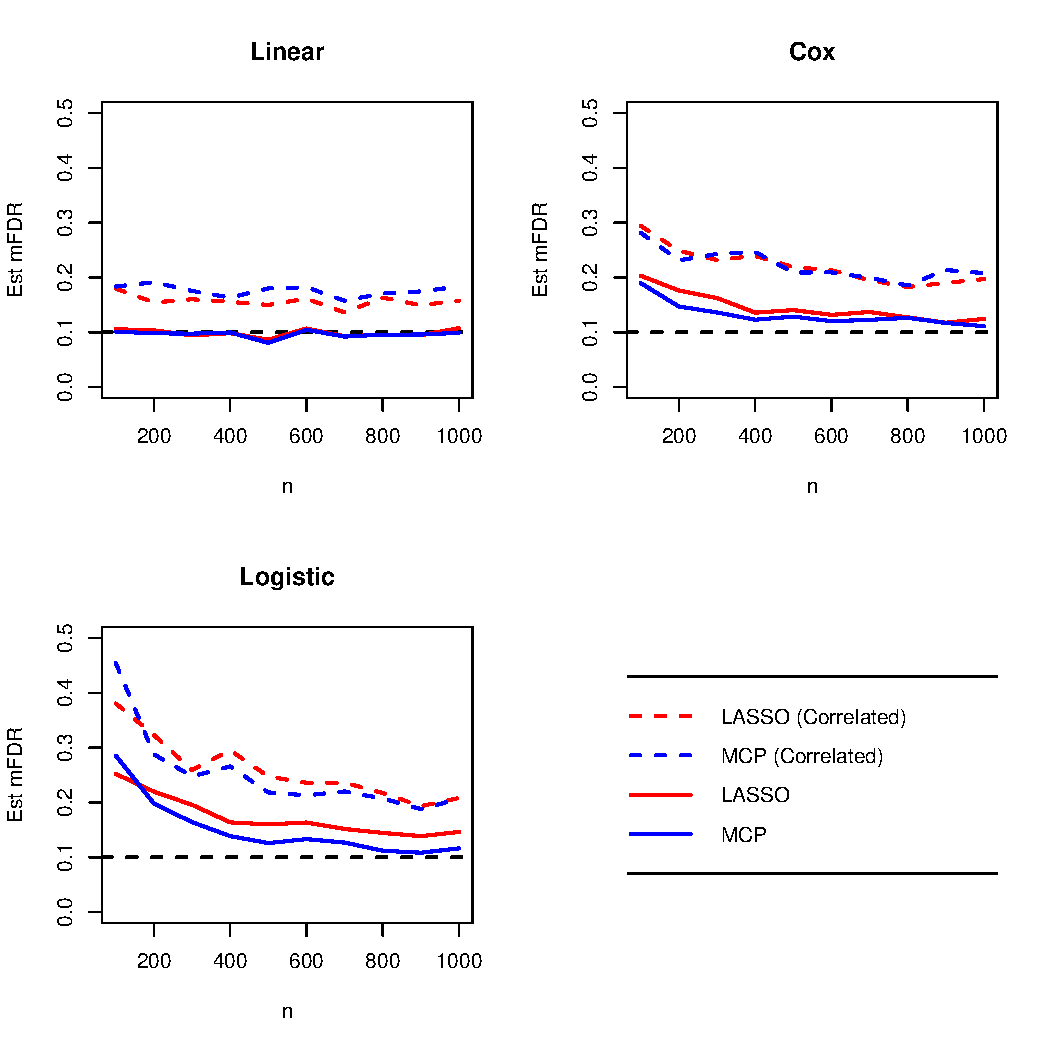
\includegraphics[scale = .5]{converge.pdf}
  \caption{Inaccuracy of the mFDR estimator }
\end{figure}

We can see that the MFDR estimator tends to be conservative with its conservatism decreasing as $n$ increases.  In the case of independent false variables the estimator approaches the nominal marginal false discovery rate as $n$ increases.  This convergence occurs nearly instantaneously linear regression, with the estimator being very accurate even at $n=100$, it occurs more slowly for logistic and Cox regression with the estimator being very slightly conservative even when $n > 500$.

Correlation between noise variables induces a conservative bias that is not remedied by increases in sample size.  This issue is not unique to mFDR as many methods for controlling false discovery rates are conservative in correlated settings.  Even with its conservative nature, mFDR remains a useful tool in guarding against false discoveries.  

Finally, we observe that the MCP penalty tends to have slightly better accuracy than the lasso penalty, particularly in the logistic and Cox regression settings.  This is likely due to the MCP's tendency towards less biased coefficient estimates which allows for assumption A3 to be more easily achieved.

\subsection{Inaccuracy and censoring}

Cox regression poses additional accuracy concerns because of censoring. In Cox Regression the individual covariate distributions may change over time depending upon each variable's relationship to censoring mechanism.  If a variable is related to censoring its distribution will drift over time as certain values are disproportionately removed from the risk set. This has the potential to induce to correlations between noise variables, in violation of assumption A2.

In this simulation study we assess the influence of variables being associated with the censoring mechanism on the accuracy of the mFDR estimator in two scenarios.  In each scenario censoring times are generated from exponential distributions with $\theta_{i} = \exp(\x_i^T \bg)$. In scenario A, $\bg_A = (0, 0, 0, 0, 1, -1, 1, -1, 0, \ldots, 0) $; while in scenario B, $\bg_B = (0, \ldots, 0) )$.  By design, each of these scenarios results in approximately 50\% of the observations being censored.  The same set of $n = 100$ true failure times is used for both scenarios and are generated from independent exponential distributions with rate parameter $\theta_i = \exp(\x_i^T \bb)$, where $\beta_{1:4} = 1$ and $\beta_{5:40} = 0$.
\begin{table}[!htb]
 \caption{Average true mFDR (10,000 simulations) when the estimated mFDR is 10\%}
\centering
\begin{tabular}{c c c}
  \hline
 & lasso & MCP   \\  [0.5ex]
  \hline \hline 
  Scenario A & 1.02\% & 6.72\% \\ 
  Scenario B &  1.33\% & 7.31\% \\ 
   \hline
\end{tabular}
\end{table}

We see that correlation induced between noise variables in scenario A leads to a more conservative mFDR estimator.  However, despite the very strong relationship noise variables had with censoring the impact on mFDR is relatively small.

\subsection{Comparison with other methods}

In this simulation study we assess the rate at which true variables are selected when attempting to control the marginal false discovery rate at 10\%. We compare the true selection rate in both low($p = 100$) and high($p=1000$) dimensional settings for a variety of effect sizes. In both settings $n = 400$, with ten variables are truly related to the outcome with $\beta_{1:10} = b$ where $b$ is varied throughout the study.  

We assess the following methods: The first is our proposed method, which uses estimated mFDR to select $\lambda$.  The second is an approach based upon sample splitting \citep{Sample_Splitting} where we first fit a lasso regression model using half of the data to select the top 20 variables, then we use the remaining data to fit a unpenalized regression model on the selected variables.  Using the unpenalized model we can conduct traditional hypothesis tests on the regression coefficients and apply the Benjamini-Hochberg procedure \citep{BH_1995} to control the false discovery rate. We use our first step to select 20 variables to ensure the second stage model contains 10 events per variable, which is essential for the hypothesis tests done on the model coefficients to have the proper type I error \citep{peduzzi_epv}. The third is the covariance testing approach of \citet{CovTest}, which we use in conjunction with the forward stopping rules proposed by \citet{GSell2016} to control the false discovery rate. The final approach uses 10-fold cross validation to select the $\lambda$ value which minimizes deviance.

\begin{figure} [!htb]
 \centering
  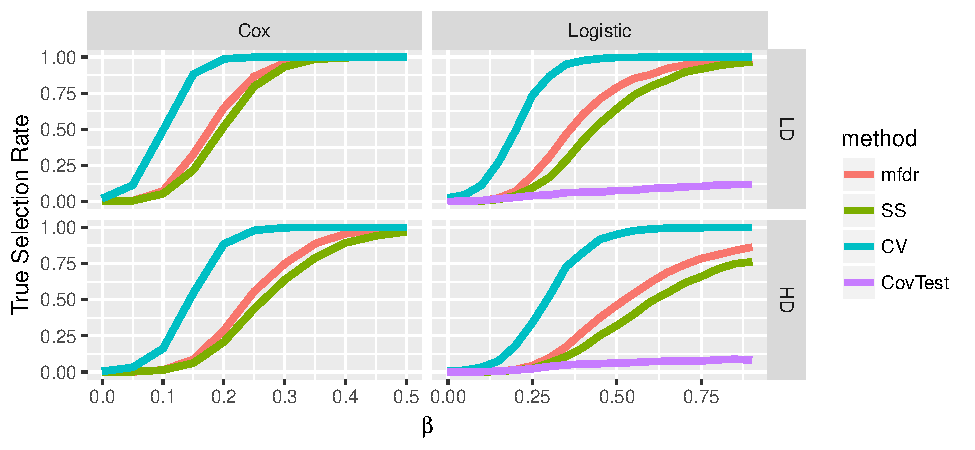
\includegraphics[scale = .5]{power.pdf}
  \caption{The average proportion of true variables selected across 1,000 simulation iterations by each method is plotted as a function of $\beta$ }
\end{figure}

In both the low-dimensional and high-dimensional settings the mFDR approach is able to select a greater proportion of the truly non-zero variables for every value of $b$ when compared to the covariance testing and the sample splitting approaches. Cross validation is able to select an even higher proportion of true variables, however it does not control the false discovery of its selections. While the other approaches all had empirical false discovery rates well under 10\% throughout our simulations, we observed cross validation to have empirical false discovery rates as high as 80\% in some scenarios.  We make the caveat that the covariance testing procedure for logistic regression is currently considered by its creators to be experimental.  Additionally, the procedure has not yet been implemented for Cox regression.

\section{Case Studies}

\subsection{Lung Cancer Survival and Gene Expression}
\citet{Shedden2008} studied the survival of 442 early-stage lung cancer subjects. Researchers collected high-dimensional gene expression data consisting of 22,283 genetic features and additional clinical covariates of age, race, gender, smoking history, cancer grade, and whether or not the subject received adjuvent chemotherapy.  

In our analysis we aim to select of important genetic features while controlling the marginal false discovery rate.  We use a penalized Cox Proportional Hazards regression model that allows for all of the clinical covariates to enter the model unpenalized while using the sparsity introduced by penalization to select additional genetic features.  We target an mFDR of 10\% and explore both the lasso and MCP penalties, while comparing our results to those of other methods.

\begin{figure} [!htb]
 \centering
  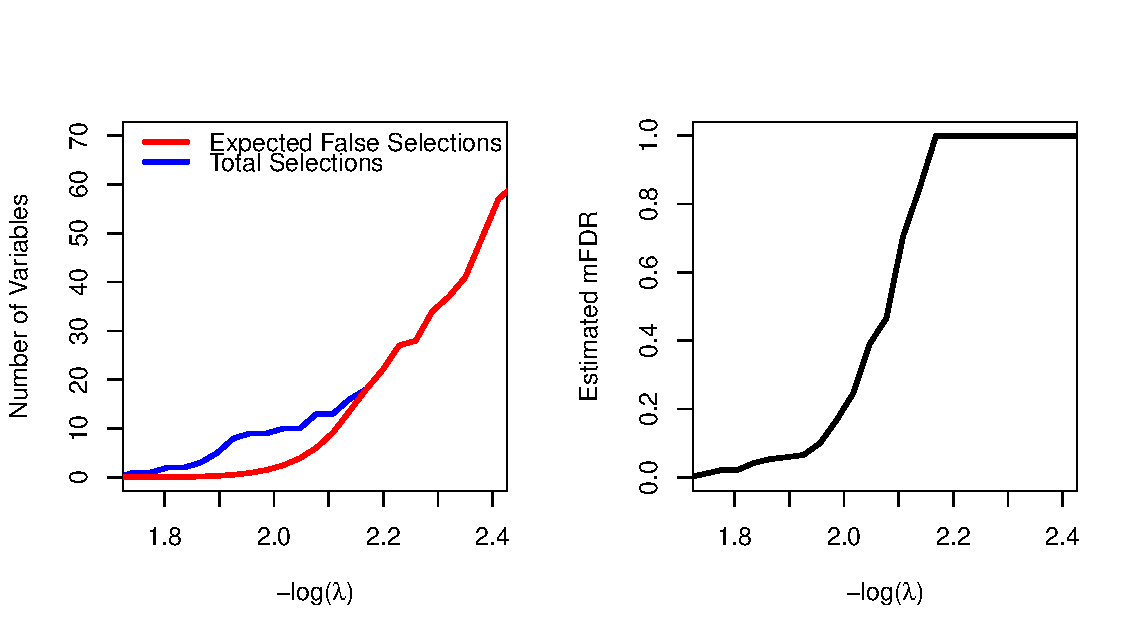
\includegraphics[scale = .7]{Shedden.pdf}
  \caption{\label{Fig:Shedden} The estimated mFDR compared to the total number of features selected and how many expected false selections were made at each $\lambda$ value}
\end{figure}

In Figure~\ref{Fig:Shedden} we see a discrepancy between the total number of selections and the expected number of false selections for many values of $\lambda$, this indicates that some of the genetic features in the dataset are likely to be truly related to survival. 

Using a target 10\% mFDR leads to a choice of $\lambda$ that selects, 9 genetic features when using the lasso penalty. Using cross validation results in the selection of a much smaller $\lambda$ that corresponds to the selection of 28 genetic features however the estimated mFDR at this choice of $\lambda$ is 100\% indicating that we likely have not controlled the number of false selections. Using the MCP penalty, the targeted 10\% mFDR threshold results in the selection of only 2 genetic features and cross validation selects 26 genetic features.  This is reflective of the tendency of the MCP penalty to lead to more parsimonious models.

When analyzing the data using the approach proposed by \citet{Meinshausen2009}, which repeatedly performs sample splitting using a large number random splits, we are unable to select any genetic features. Additionally the current version of the covTest package, which is used to carry out the covariance testing approach, currently does not accommodate survival data.

Another popular method used for gene selection is to univariately test each genetic feature and adjust the test results to control the false discovery rate.  For comparison purposes we applied this approach to the Shedden data in two ways.  The first fits a univariate Cox regression model to each genetic feature and tests the features effect on survival.  The second is similar except with each model adjusting for clinical covariates in addition to the single genetic feature.  Using the Benjamini-Hochberg procedure to control the false discovery rate at 10\%, these two univariate testing approaches result in the selection of 862 and 803 features respectively.  These results are illustrative of the difference between model based approaches and large scale univariate testing.  Univariate approaches tends select many features from a few groups that are correlated with each other, adding a degree of redundancy to the results.  Modeling approaches tend to instead select a single representative from each group of correlated features.  

\subsection{Lung Cancer Status Among Smokers}
\citet{Spira2007} collected RNA expression data from histologically normal bronchial epitheliums of $n = 192$ smokers of which 102 had developed lung cancer and 90 had not developed lung cancer.  We are interested identifying genetic features that are indicative of whether or not a smoker has lung cancer.  For our analysis we a penalized fit logistic regression model using both the lasso and MCP penalties. We compare the results at $\lambda$ values chosen using estimated MFDR, cross validation, and the covariance test.  We also compare these model based approaches to the traditional univariate approach with false discovery rate control.

\begin{table}[ht]
\centering
\begin{tabular}{c|rrr|rrr}
  \hline
 & & lasso & & & MCP & \\
 \hline
$\lambda$ & EF & S & mFDR & EF & S & mFDR \\ 
  \hline
0.2041 & 0.00 &   0 & 0.00 & 0.00 &   0 & 0.00 \\ 
  0.1980 & 0.00 &   2 & 0.00 & 0.00 &   2 & 0.00 \\ 
  0.1921 & 0.00 &   4 & 0.00 & 0.00 &   2 & 0.00 \\ 
  0.1864 & 0.00 &   6 & 0.00 & 0.00 &   3 & 0.00 \\ 
  0.1809 & 0.01 &   6 & 0.00 & 0.01 &   4 & 0.00 \\ 
  0.1755 & 0.02 &   6 & 0.00 & 0.02 &   4 & 0.01 \\ 
  0.1702 & 0.04 &   6 & 0.01 & 0.04 &   4 & 0.01 \\ 
  0.1652 & 0.08 &   8 & 0.01 & 0.08 &   5 & 0.02 \\ 
  0.1602 & 0.15 &   9 & 0.02 & 0.14 &   5 & 0.03 \\ 
  0.1555 & 0.27 &   8 & 0.03 & 0.25 &   5 & 0.05 \\ 
  0.1508 & 0.47 &   8 & 0.06 & 0.42 &   5 & 0.08 \\ 
  0.1463 & 0.78 &  10 & 0.08 & 0.69 &   5 & 0.14 \\ 
  0.1420 & 1.27 &  10 & 0.13 & 1.10 &   5 & 0.22 \\ 
  0.1377 & 2.00 &  11 & 0.18 & 1.72 &   8 & 0.22 \\ 
  0.1336 & 3.10 &  13 & 0.24 & 2.69 &   7 & 0.38 \\ 
   \hline
\end{tabular}
 \caption{The estimated mFDR results for 15 values of the $\lambda$ sequence which straddle our target mFDR}
\end{table}

Using the lasso penalty and a target MFDR threshold of 10\% we select a $\lambda$ value of 0.146 corresponding to the selection of 10 features.  Cross Validation selects a $\lambda$ of 0.056 corresponding to the selection of 40 features.  The estimated FIR at the $\lambda$ chosen by cross validation is 100\%, indicating that we cannot be confident that the number of false selections has been controlled.  If instead we use the MCP penalty we select a $\lambda$ value of 0.1508, corresponding to 5 features, when targeting 10\% FIR; and using cross validation we select a $\lambda$ value of 0.0666, corresponding to 14 features.  Again the estimated MFDR at the $\lambda$ chosen by cross validation is 100\%.  

The sample splitting approach, using 100 random splits, does not select any features after controlling the false discovery rate. Only a single genetic feature reached the second stage in at at least half of the splits and its median p-value was not significant. 

The Covariance Testing approach also does not select any features.  The first variable to enter the model has a p-value of 0.475 and when the ForwardStop procedure is applied we cannot proceed past the intercept only model if without the false discovery rate exceeding 10\%.

Finally we applied the univariate testing approach to these data in two ways.  The first uses t-tests to assess the difference in expression for each genetic feature for the two groups while controlling the false discovery rate at 10\% using the Benjamini$-$Hochberg procedure.  This procedure ends up selecting selecting 2,965 genetic features. An alternative approach is to use univariate logistic regression instead of t-tests in the aforementioned procedure, which leads to selection of 2,833 genetic features.  This is illustrates the tendency of model based approaches to select only a single feature from a correlated group, while univariate approaches select all of the features within correlated groups. 

\section{Discussion}
Quantifying the reliability of feature selections when using penalized regression models is valuable when analyzing high dimensional data and using the false inclusion rate estimator proposed in this paper is one way of accomplishing this.  Unlike other approaches that have a similar goal, such as sample splitting or the covariance test, mFDR uses a more relaxed definition of a false discovery which does not limit variables with $\beta_j = 0$ but rather only limits variables that are truly noise in the sense that they are completely independent of outcome regardless of which other variables are in the model.  The simulation comparisons in this paper demonstrate that with this definition mFDR has higher power to detect features than other methods.  The estimator tends to be conservative compared to the true false inclusion rate but our simulations and case studies suggest that it is a useful tool despite being conservative.

The mFDR estimator is currently implemented in R in the \text{ncvreg} package \citep{Breheny2011} using the \text{mFDR} function.  The function takes in a model it and provides estimates of the expected number of false discoveries, as well as the mFDR for each value of the $\lambda$ sequence used in fitting the model.  The function accommodates lasso, MCP, SCAD, elastic net, and MNet \citep{Huang2016} penalties and provides a convenient model summary measure for penalized regression models.

In the simulations and case studies the sample splitting approach had to be coded manually due to existing software being unable to handle logistic and survival models.  The covariance testing approach was implemented using the \text{CovTest} package \citep{CovTest} and the \text{forwardStop} function of the \text{SelectiveInference} package \citep{Selective_Inference}.  The authors of the package caution that the approach is experimental for logistic regression.  This lack of software adds to the appeal of using mFDR as a means to assess feature selection reliability after fitting penalized regression model with a binary or survival outcome.
